\documentclass{article}
\usepackage[UTF8]{ctex}
\usepackage[T1]{fontenc}
\usepackage[utf8]{inputenc}
\usepackage{titlesec}
\usepackage[colorlinks, linkcolor = black]{hyperref}
\usepackage{float}
\usepackage{xcolor}
\usepackage{tikz}
\usepackage{subfigure}
\usetikzlibrary{positioning}
\usetikzlibrary[arrows, shapes, chains]

\titleformat{\section}[block]{\LARGE\scshape}{\arabic{section}}{1em}{}[]

\title{Homework 1}
\author{PB17000297 罗晏宸}
\date{March 1 2020}

\begin{document}
\maketitle

\section{Exercise 3.6}
对以下问题给出完整的形式化。选择的形式化方法要足够精确以便于实现。
\subparagraph{a}
只用四种颜色对平面地图着色,要求每两个相邻的地区不能具有相同的颜色。
\subparagraph{b}
屋子里有只3英尺高的猴子,离地8英尺的屋顶上挂着一串香蕉。猴子想吃香蕉。屋子里有两个可叠放、可移动、可攀爬的3英尺高的箱子。
\subparagraph{d}
有三个水壶,容量分别为12加仑、8加仑和3加仑,还有一个放液嘴。可以把水壶装满或者倒空,从一个壶倒进另一个壶或者倒在地上。请量出刚好1加仑水。

\paragraph{解}
\subparagraph{a}
\begin{itemize}
    \item 初始状态:所有地区均未被着色
    \item 可能的行动:给定一个状态,对其中一个未被着色的地区分配一种和与其相邻的已着色地区都不相同的颜色
    \item 转移模型:从一个状态达到一个已着色地区数加一的状态
    \item 目标测试:所有地区都已被着色,且每两个相邻的地区都不具有相同的颜色
    \item 路径耗散:总共的着色次数
\end{itemize}
\subparagraph{b}
\begin{itemize}
    \item 初始状态:箱子未被叠放,猴子活动在地面上
    \item 可能的行动:在(某一高度上)移动,移动一个(猴子不站立在其上的)箱子,(在两个箱子均放置在地面上时)叠放两个箱子,跳上一个(与猴子在同一高度的)箱子,从一个箱子上跳下,(在猴子最高处达到或超过香蕉高度时)摘取香蕉
    \item 转移模型:从一个状态达到另一个状态,猴子以及两个箱子彼此相对位置改变
    \item 目标测试:猴子摘取到香蕉
    \item 路径耗散:行动次数
\end{itemize}
\subparagraph{d}
\begin{itemize}
    \item 初始状态:三个水壶均为空,记为三元组$(0,\,0,\,0)$
    \item 可能的行动:把其中一个水壶倒满,把其中一个水壶倒空,从一个壶倒进另一个壶
    \item 转移模型:对于状态$(x_1,\,x_2,\,x_3)$,把一个水壶倒满后可以达到$(3,\,x_2,\,x_3)$、$(x_1,\,8,\,x_3)$或$(x_1,\,x_2,\,12)$,把一个水壶倒空后可以达到$(0,\,x_2,\,x_3)$、$(x_1,\,0,\,x_3)$或$(x_1,\,x_2,\,0)$,从一个壶$i(i = 1,2,3)$倒进另一个壶$j(j = 1,2,3,\, j \neq i)$后可以达到 $x'_i = 0,\, x'_j = x_i + x_j,\ (x_i + x_j \leq C_j)$ 或 $x'_i = x_i + x_j - C_j,\, x'_j = C_j,\ (x_i + x_j > C_j)$ ,其中$C_j$是壶$j$的容量
    \item 目标测试:其中一个水壶中刚好有一加仑水
    \item 路径耗散:行动次数
\end{itemize}

\section{Exercise 3.9}
\textbf{传教士和野人}问题。三个传教士和三个野人在河的一岸,有一条能载一个人或者两个人的船。请设法使所有人都渡到河的另一岸,要求在任何地方野人数都不能多于传教士的人数,这个问题在AI领域中很有名,是因为它是第一个从分析的观点探讨问题形式化的论文的主题(Amarel, 1968)。
\subparagraph{a}
请对该问题进行详细形式化,只描述确保该问题求解所必需的特性。画出完整的状态空间图。
\subparagraph{b}
应用合适的搜索算法求出该问题的最优解。对于这个问题检查重复状态是个好主意吗?
\subparagraph{c}
这个问题的状态空间很简单,你认为是什么导致人们求解它很困难?

\paragraph{解}
\subparagraph{a}
\begin{itemize}
    \item 状态:用三元组$(M,\,C,\,B)$表示,其中$M$表示左岸(不妨将开始六人所在的河岸设为左岸)的传教士人数,$C$表示左岸野人数,$B = L$表示船在左岸,$B = R$表示船在右岸。因此可能的状态有$4 \times 4 \times 2 = 32$个,其中受限于在任何地方野人数都不能多于传教士人数的要求,有12个状态不合法,另有5个状态在问题中不存在,因此总的状态有$15$个。
    \item 初始状态:三个传教士和三个野人在河的左岸,记为$(3, 3, L)$
    \item 行动:用$T_{M,C}$表示$M$个传教士和$C$个野人划船去另一岸。因此可能的行动有$T_{0,1},\,T_{0,2},\,T_{1,0},\,T_{1,1},\,T_{2,0}$共5种
    \item 转移模型:对于状态$(M,\,C,\,B = L/R)$,行动$T_{0,1},\,T_{0,2},\,T_{1,0},\,T_{1,1},\,T_{2,0}$分别转移到$(M,\,C - 1,\,B = R/L),\,(M,\,C - 2,\,B = R/L),\,(M - 1,\,C,\,B = R/L),\,(M - 1,\,C - 1,\,B = R/L),\,(M - 2,\,C,\,B = R/L)$,完整的状态空间如图\ref{figure:1}所示
    \item 目标测试:达到状态$(3, 3, R)$
    \item 路径耗散:划船行动的次数
\end{itemize}
\begin{figure}[H]
    \centering
    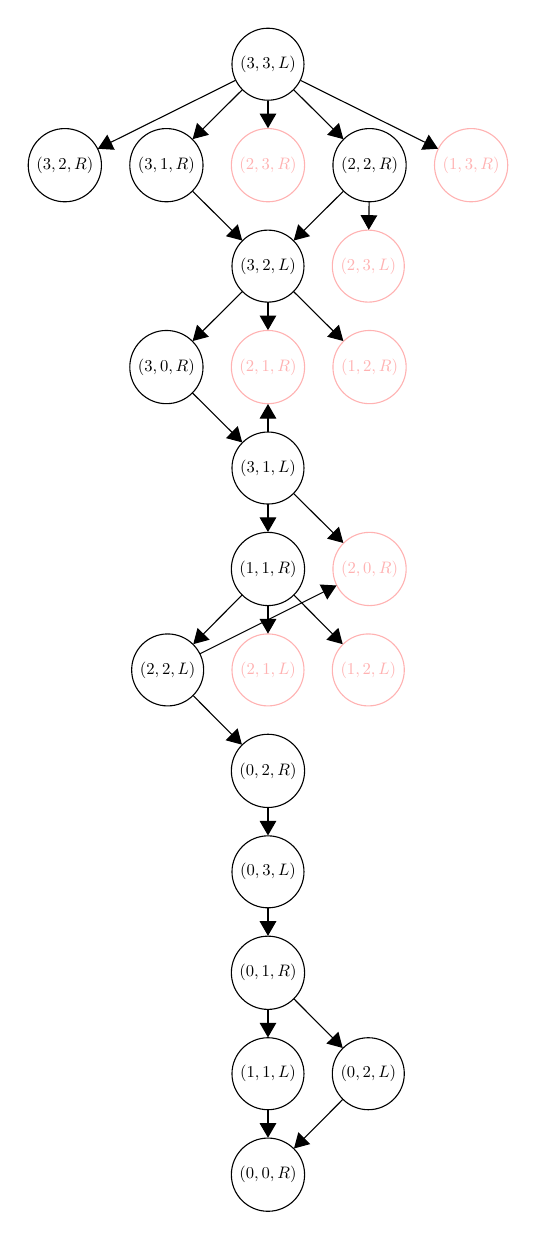
\begin{tikzpicture}[node distance = 1.0em]
        \tikzstyle{state} = [scale = 0.6, circle, draw=black, text ragged];
        \tikzstyle{illegal} = [scale = 0.6, circle, draw=red!30!white, text ragged, red!30!white]
        \node [state] (S0) {$(3, 3, L)$};

        \node [illegal, below = of S0] (S1) {$(2, 3, R)$};
        \node [state, left = of S1] (S2) {$(3, 1, R)$};
        \node [state, right = of S1] (S3) {$(2, 2, R)$};
        \node [state, left = of S2] (S4) {$(3, 2, R)$};
        \node [illegal, right = of S3] (S5) {$(1, 3, R)$};

        \node [state, below = of S1] (S6) {$(3, 2, L)$};
        \node [illegal, right = of S6] (S7) {$(2, 3, L)$};

        \node [illegal, below = of S6] (S8) {$(2, 1, R)$};
        \node [state, left = of S8] (S9) {$(3, 0, R)$};
        \node [illegal, right = of S8] (S10) {$(1, 2, R)$};

        \node [state, below = of S8] (S11) {$(3, 1, L)$};

        \node [state, below = of S11] (S12) {$(1, 1, R)$};
        \node [illegal, right = of S12] (S13) {$(2, 0, R)$};


        \node [illegal, below = of S12] (S14) {$(2, 1, L)$};
        \node [state, left = of S14] (S15) {$(2, 2, L)$};
        \node [illegal, right = of S14] (S16) {$(1, 2, L)$};

        \node [state, below = of S14] (S17) {$(0, 2, R)$};

        \node [state, below = of S17] (S18) {$(0, 3, L)$};

        \node [state, below = of S18] (S19) {$(0, 1, R)$};

        \node [state, below = of S19] (S20) {$(1, 1, L)$};
        \node [state, right = of S20] (S21) {$(0, 2, L)$};

        \node [state, below = of S20] (S22) {$(0, 0, R)$};

        \foreach \i in {1, ..., 5}
            \draw [-triangle 60] (S0) to (S\i);
        \foreach \i/\j in {2/6, 3/6, 3/7}
            \draw [-triangle 60] (S\i) to (S\j);
        \foreach \i in {8, 9, 10}
            \draw [-triangle 60] (S6) to (S\i);
        \draw [-triangle 60] (S9) to (S11);
        \foreach \i in {12, 13, 8}
            \draw [-triangle 60] (S11) to (S\i);
        \foreach \i in {14, 15, 16}
            \draw [-triangle 60] (S12) to (S\i);
        \foreach \i in {17, 13}
            \draw [-triangle 60] (S15) to (S\i);
        \foreach \i/\j in {17/18, 18/19, 19/20, 19/21, 20/22, 21/22}
            \draw [-triangle 60] (S\i) to (S\j);
    \end{tikzpicture}
    \caption{传教士和野人问题的状态空间}
    \label{figure:1}
\end{figure}
\subparagraph{b}
由于状态空间比较简单,应用宽度优先搜索,搜索过程如图\ref{figure:2}所示
\begin{figure}
    \centering
    \subfigure{
        
\begin{tikzpicture}[node distance = 0.3em]
            \tikzstyle{state} = [scale = 0.25, circle, draw=black, text ragged];
            \tikzstyle{illegal} = [scale = 0.25, circle, draw=red!30!white, text ragged, red!30!white]
            \node [state] (S0) {$(3, 3, L)$};
        \end{tikzpicture}
    }
    \subfigure{
        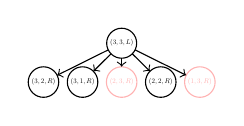
\begin{tikzpicture}[node distance = 0.3em]
            \tikzstyle{state} = [scale = 0.25, circle, draw=black, text ragged];
            \tikzstyle{illegal} = [scale = 0.25, circle, draw=red!30!white, text ragged, red!30!white]
            \node [state] (S0) {$(3, 3, L)$};

            \node [illegal, below = of S0] (S1) {$(2, 3, R)$};
            \node [state, left = of S1] (S2) {$(3, 1, R)$};
            \node [state, right = of S1] (S3) {$(2, 2, R)$};
            \node [state, left = of S2] (S4) {$(3, 2, R)$};
            \node [illegal, right = of S3] (S5) {$(1, 3, R)$};

            \foreach \i in {1, ..., 5}
                \draw [->] (S0) to (S\i);

        \end{tikzpicture}
    }
    \subfigure{
        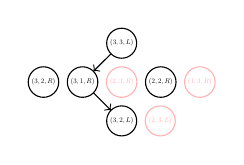
\begin{tikzpicture}[node distance = 0.3em]
            \tikzstyle{state} = [scale = 0.25, circle, draw=black, text ragged];
            \tikzstyle{illegal} = [scale = 0.25, circle, draw=red!30!white, text ragged, red!30!white]
            \node [state] (S0) {$(3, 3, L)$};

            \node [illegal, below = of S0] (S1) {$(2, 3, R)$};
            \node [state, left = of S1] (S2) {$(3, 1, R)$};
            \node [state, right = of S1] (S3) {$(2, 2, R)$};
            \node [state, left = of S2] (S4) {$(3, 2, R)$};
            \node [illegal, right = of S3] (S5) {$(1, 3, R)$};

            \node [state, below = of S1] (S6) {$(3, 2, L)$};
            \node [illegal, right = of S6] (S7) {$(2, 3, L)$};

            \draw [->] (S0) to (S2);
            \draw [->] (S2) to (S6);
        \end{tikzpicture}
    }
    \subfigure{
        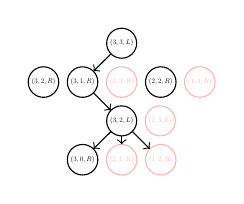
\begin{tikzpicture}[node distance = 0.3em]
            \tikzstyle{state} = [scale = 0.25, circle, draw=black, text ragged];
            \tikzstyle{illegal} = [scale = 0.25, circle, draw=red!30!white, text ragged, red!30!white]
            \node [state] (S0) {$(3, 3, L)$};

            \node [illegal, below = of S0] (S1) {$(2, 3, R)$};
            \node [state, left = of S1] (S2) {$(3, 1, R)$};
            \node [state, right = of S1] (S3) {$(2, 2, R)$};
            \node [state, left = of S2] (S4) {$(3, 2, R)$};
            \node [illegal, right = of S3] (S5) {$(1, 3, R)$};

            \node [state, below = of S1] (S6) {$(3, 2, L)$};
            \node [illegal, right = of S6] (S7) {$(2, 3, L)$};

            \node [illegal, below = of S6] (S8) {$(2, 1, R)$};
            \node [state, left = of S8] (S9) {$(3, 0, R)$};
            \node [illegal, right = of S8] (S10) {$(1, 2, R)$};


            \draw [->] (S0) to (S2);
            \draw [->] (S2) to (S6);
            \foreach \i in {8, 9, 10}
                \draw [->] (S6) to (S\i);
        \end{tikzpicture}
    }

    \subfigure{
        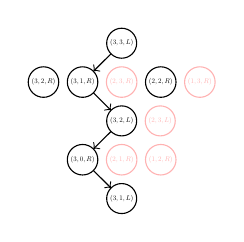
\begin{tikzpicture}[node distance = 0.3em]
            \tikzstyle{state} = [scale = 0.25, circle, draw=black, text ragged];
            \tikzstyle{illegal} = [scale = 0.25, circle, draw=red!30!white, text ragged, red!30!white]
            \node [state] (S0) {$(3, 3, L)$};

            \node [illegal, below = of S0] (S1) {$(2, 3, R)$};
            \node [state, left = of S1] (S2) {$(3, 1, R)$};
            \node [state, right = of S1] (S3) {$(2, 2, R)$};
            \node [state, left = of S2] (S4) {$(3, 2, R)$};
            \node [illegal, right = of S3] (S5) {$(1, 3, R)$};

            \node [state, below = of S1] (S6) {$(3, 2, L)$};
            \node [illegal, right = of S6] (S7) {$(2, 3, L)$};

            \node [illegal, below = of S6] (S8) {$(2, 1, R)$};
            \node [state, left = of S8] (S9) {$(3, 0, R)$};
            \node [illegal, right = of S8] (S10) {$(1, 2, R)$};

            \node [state, below = of S8] (S11) {$(3, 1, L)$};


            \draw [->] (S0) to (S2);
            \draw [->] (S2) to (S6);
            \draw [->] (S6) to (S9);
            \draw [->] (S9) to (S11);
        \end{tikzpicture}
    }
    \subfigure{
        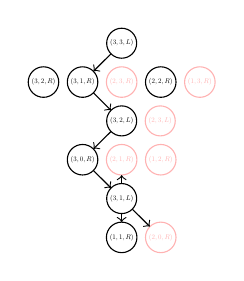
\begin{tikzpicture}[node distance = 0.3em]
            \tikzstyle{state} = [scale = 0.25, circle, draw=black, text ragged];
            \tikzstyle{illegal} = [scale = 0.25, circle, draw=red!30!white, text ragged, red!30!white]
            \node [state] (S0) {$(3, 3, L)$};

            \node [illegal, below = of S0] (S1) {$(2, 3, R)$};
            \node [state, left = of S1] (S2) {$(3, 1, R)$};
            \node [state, right = of S1] (S3) {$(2, 2, R)$};
            \node [state, left = of S2] (S4) {$(3, 2, R)$};
            \node [illegal, right = of S3] (S5) {$(1, 3, R)$};

            \node [state, below = of S1] (S6) {$(3, 2, L)$};
            \node [illegal, right = of S6] (S7) {$(2, 3, L)$};

            \node [illegal, below = of S6] (S8) {$(2, 1, R)$};
            \node [state, left = of S8] (S9) {$(3, 0, R)$};
            \node [illegal, right = of S8] (S10) {$(1, 2, R)$};

            \node [state, below = of S8] (S11) {$(3, 1, L)$};

            \node [state, below = of S11] (S12) {$(1, 1, R)$};
            \node [illegal, right = of S12] (S13) {$(2, 0, R)$};

            \draw [->] (S0) to (S2);
            \draw [->] (S2) to (S6);
            \draw [->] (S6) to (S9);
            \draw [->] (S9) to (S11);
            \foreach \i in {12, 13, 8}
                \draw [->] (S11) to (S\i);
        \end{tikzpicture}
    }
    \subfigure{
        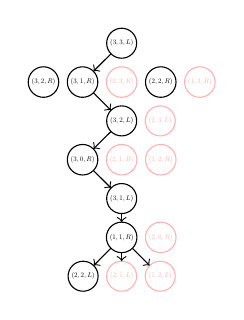
\begin{tikzpicture}[node distance = 0.3em]
            \tikzstyle{state} = [scale = 0.25, circle, draw=black, text ragged];
            \tikzstyle{illegal} = [scale = 0.25, circle, draw=red!30!white, text ragged, red!30!white]
            \node [state] (S0) {$(3, 3, L)$};

            \node [illegal, below = of S0] (S1) {$(2, 3, R)$};
            \node [state, left = of S1] (S2) {$(3, 1, R)$};
            \node [state, right = of S1] (S3) {$(2, 2, R)$};
            \node [state, left = of S2] (S4) {$(3, 2, R)$};
            \node [illegal, right = of S3] (S5) {$(1, 3, R)$};

            \node [state, below = of S1] (S6) {$(3, 2, L)$};
            \node [illegal, right = of S6] (S7) {$(2, 3, L)$};

            \node [illegal, below = of S6] (S8) {$(2, 1, R)$};
            \node [state, left = of S8] (S9) {$(3, 0, R)$};
            \node [illegal, right = of S8] (S10) {$(1, 2, R)$};

            \node [state, below = of S8] (S11) {$(3, 1, L)$};

            \node [state, below = of S11] (S12) {$(1, 1, R)$};
            \node [illegal, right = of S12] (S13) {$(2, 0, R)$};


            \node [illegal, below = of S12] (S14) {$(2, 1, L)$};
            \node [state, left = of S14] (S15) {$(2, 2, L)$};
            \node [illegal, right = of S14] (S16) {$(1, 2, L)$};

            \draw [->] (S0) to (S2);
            \draw [->] (S2) to (S6);
            \draw [->] (S6) to (S9);
            \draw [->] (S9) to (S11);
            \draw [->] (S11) to (S12);
            \foreach \i in {14, 15, 16}
                \draw [->] (S12) to (S\i);
        \end{tikzpicture}
    }
    \subfigure{
        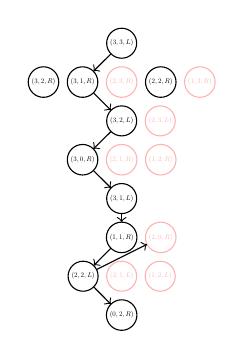
\begin{tikzpicture}[node distance = 0.3em]
            \tikzstyle{state} = [scale = 0.25, circle, draw=black, text ragged];
            \tikzstyle{illegal} = [scale = 0.25, circle, draw=red!30!white, text ragged, red!30!white]
            \node [state] (S0) {$(3, 3, L)$};

            \node [illegal, below = of S0] (S1) {$(2, 3, R)$};
            \node [state, left = of S1] (S2) {$(3, 1, R)$};
            \node [state, right = of S1] (S3) {$(2, 2, R)$};
            \node [state, left = of S2] (S4) {$(3, 2, R)$};
            \node [illegal, right = of S3] (S5) {$(1, 3, R)$};

            \node [state, below = of S1] (S6) {$(3, 2, L)$};
            \node [illegal, right = of S6] (S7) {$(2, 3, L)$};

            \node [illegal, below = of S6] (S8) {$(2, 1, R)$};
            \node [state, left = of S8] (S9) {$(3, 0, R)$};
            \node [illegal, right = of S8] (S10) {$(1, 2, R)$};

            \node [state, below = of S8] (S11) {$(3, 1, L)$};

            \node [state, below = of S11] (S12) {$(1, 1, R)$};
            \node [illegal, right = of S12] (S13) {$(2, 0, R)$};


            \node [illegal, below = of S12] (S14) {$(2, 1, L)$};
            \node [state, left = of S14] (S15) {$(2, 2, L)$};
            \node [illegal, right = of S14] (S16) {$(1, 2, L)$};

            \node [state, below = of S14] (S17) {$(0, 2, R)$};

            \draw [->] (S0) to (S2);
            \draw [->] (S2) to (S6);
            \draw [->] (S6) to (S9);
            \draw [->] (S9) to (S11);
            \draw [->] (S11) to (S12);
            \draw [->] (S12) to (S15);
            \foreach \i in {17, 13}
                \draw [->] (S15) to (S\i);
        \end{tikzpicture}
    }

    \subfigure{
        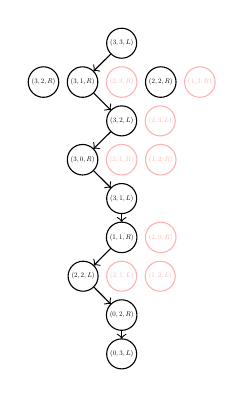
\begin{tikzpicture}[node distance = 0.3em]
            \tikzstyle{state} = [scale = 0.25, circle, draw=black, text ragged];
            \tikzstyle{illegal} = [scale = 0.25, circle, draw=red!30!white, text ragged, red!30!white]
            \node [state] (S0) {$(3, 3, L)$};

            \node [illegal, below = of S0] (S1) {$(2, 3, R)$};
            \node [state, left = of S1] (S2) {$(3, 1, R)$};
            \node [state, right = of S1] (S3) {$(2, 2, R)$};
            \node [state, left = of S2] (S4) {$(3, 2, R)$};
            \node [illegal, right = of S3] (S5) {$(1, 3, R)$};

            \node [state, below = of S1] (S6) {$(3, 2, L)$};
            \node [illegal, right = of S6] (S7) {$(2, 3, L)$};

            \node [illegal, below = of S6] (S8) {$(2, 1, R)$};
            \node [state, left = of S8] (S9) {$(3, 0, R)$};
            \node [illegal, right = of S8] (S10) {$(1, 2, R)$};

            \node [state, below = of S8] (S11) {$(3, 1, L)$};

            \node [state, below = of S11] (S12) {$(1, 1, R)$};
            \node [illegal, right = of S12] (S13) {$(2, 0, R)$};


            \node [illegal, below = of S12] (S14) {$(2, 1, L)$};
            \node [state, left = of S14] (S15) {$(2, 2, L)$};
            \node [illegal, right = of S14] (S16) {$(1, 2, L)$};

            \node [state, below = of S14] (S17) {$(0, 2, R)$};

            \node [state, below = of S17] (S18) {$(0, 3, L)$};

            \draw [->] (S0) to (S2);
            \draw [->] (S2) to (S6);
            \draw [->] (S6) to (S9);
            \draw [->] (S9) to (S11);
            \draw [->] (S11) to (S12);
            \draw [->] (S12) to (S15);
            \draw [->] (S15) to (S17);
            \draw [->] (S17) to (S18);
        \end{tikzpicture}
    }
    \subfigure{
        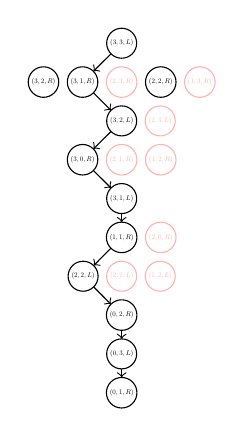
\begin{tikzpicture}[node distance = 0.3em]
            \tikzstyle{state} = [scale = 0.25, circle, draw=black, text ragged];
            \tikzstyle{illegal} = [scale = 0.25, circle, draw=red!30!white, text ragged, red!30!white]
            \node [state] (S0) {$(3, 3, L)$};

            \node [illegal, below = of S0] (S1) {$(2, 3, R)$};
            \node [state, left = of S1] (S2) {$(3, 1, R)$};
            \node [state, right = of S1] (S3) {$(2, 2, R)$};
            \node [state, left = of S2] (S4) {$(3, 2, R)$};
            \node [illegal, right = of S3] (S5) {$(1, 3, R)$};

            \node [state, below = of S1] (S6) {$(3, 2, L)$};
            \node [illegal, right = of S6] (S7) {$(2, 3, L)$};

            \node [illegal, below = of S6] (S8) {$(2, 1, R)$};
            \node [state, left = of S8] (S9) {$(3, 0, R)$};
            \node [illegal, right = of S8] (S10) {$(1, 2, R)$};

            \node [state, below = of S8] (S11) {$(3, 1, L)$};

            \node [state, below = of S11] (S12) {$(1, 1, R)$};
            \node [illegal, right = of S12] (S13) {$(2, 0, R)$};


            \node [illegal, below = of S12] (S14) {$(2, 1, L)$};
            \node [state, left = of S14] (S15) {$(2, 2, L)$};
            \node [illegal, right = of S14] (S16) {$(1, 2, L)$};

            \node [state, below = of S14] (S17) {$(0, 2, R)$};

            \node [state, below = of S17] (S18) {$(0, 3, L)$};

            \node [state, below = of S18] (S19) {$(0, 1, R)$};

            \draw [->] (S0) to (S2);
            \draw [->] (S2) to (S6);
            \draw [->] (S6) to (S9);
            \draw [->] (S9) to (S11);
            \draw [->] (S11) to (S12);
            \draw [->] (S12) to (S15);
            \draw [->] (S15) to (S17);
            \draw [->] (S17) to (S18);
            \draw [->] (S18) to (S19);
        \end{tikzpicture}
    }
    \subfigure{
        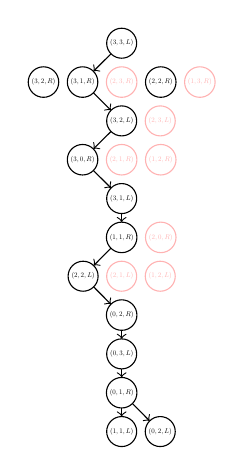
\begin{tikzpicture}[node distance = 0.3em]
            \tikzstyle{state} = [scale = 0.25, circle, draw=black, text ragged];
            \tikzstyle{illegal} = [scale = 0.25, circle, draw=red!30!white, text ragged, red!30!white]
            \node [state] (S0) {$(3, 3, L)$};

            \node [illegal, below = of S0] (S1) {$(2, 3, R)$};
            \node [state, left = of S1] (S2) {$(3, 1, R)$};
            \node [state, right = of S1] (S3) {$(2, 2, R)$};
            \node [state, left = of S2] (S4) {$(3, 2, R)$};
            \node [illegal, right = of S3] (S5) {$(1, 3, R)$};

            \node [state, below = of S1] (S6) {$(3, 2, L)$};
            \node [illegal, right = of S6] (S7) {$(2, 3, L)$};

            \node [illegal, below = of S6] (S8) {$(2, 1, R)$};
            \node [state, left = of S8] (S9) {$(3, 0, R)$};
            \node [illegal, right = of S8] (S10) {$(1, 2, R)$};

            \node [state, below = of S8] (S11) {$(3, 1, L)$};

            \node [state, below = of S11] (S12) {$(1, 1, R)$};
            \node [illegal, right = of S12] (S13) {$(2, 0, R)$};


            \node [illegal, below = of S12] (S14) {$(2, 1, L)$};
            \node [state, left = of S14] (S15) {$(2, 2, L)$};
            \node [illegal, right = of S14] (S16) {$(1, 2, L)$};

            \node [state, below = of S14] (S17) {$(0, 2, R)$};

            \node [state, below = of S17] (S18) {$(0, 3, L)$};

            \node [state, below = of S18] (S19) {$(0, 1, R)$};

            \node [state, below = of S19] (S20) {$(1, 1, L)$};
            \node [state, right = of S20] (S21) {$(0, 2, L)$};

            \draw [->] (S0) to (S2);
            \draw [->] (S2) to (S6);
            \draw [->] (S6) to (S9);
            \draw [->] (S9) to (S11);
            \draw [->] (S11) to (S12);
            \draw [->] (S12) to (S15);
            \draw [->] (S15) to (S17);
            \draw [->] (S17) to (S18);
            \draw [->] (S18) to (S19);
            \foreach \i/\j in {19/20, 19/21}
                \draw [->] (S\i) to (S\j);
        \end{tikzpicture}
    }
    \subfigure{
        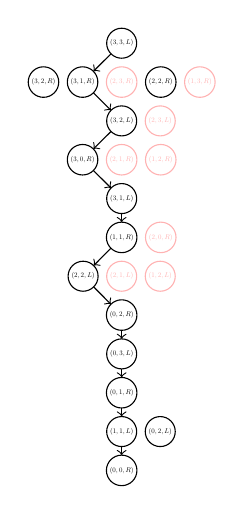
\begin{tikzpicture}[node distance = 0.3em]
            \tikzstyle{state} = [scale = 0.25, circle, draw=black, text ragged];
            \tikzstyle{illegal} = [scale = 0.25, circle, draw=red!30!white, text ragged, red!30!white]
            \node [state] (S0) {$(3, 3, L)$};

            \node [illegal, below = of S0] (S1) {$(2, 3, R)$};
            \node [state, left = of S1] (S2) {$(3, 1, R)$};
            \node [state, right = of S1] (S3) {$(2, 2, R)$};
            \node [state, left = of S2] (S4) {$(3, 2, R)$};
            \node [illegal, right = of S3] (S5) {$(1, 3, R)$};

            \node [state, below = of S1] (S6) {$(3, 2, L)$};
            \node [illegal, right = of S6] (S7) {$(2, 3, L)$};

            \node [illegal, below = of S6] (S8) {$(2, 1, R)$};
            \node [state, left = of S8] (S9) {$(3, 0, R)$};
            \node [illegal, right = of S8] (S10) {$(1, 2, R)$};

            \node [state, below = of S8] (S11) {$(3, 1, L)$};

            \node [state, below = of S11] (S12) {$(1, 1, R)$};
            \node [illegal, right = of S12] (S13) {$(2, 0, R)$};


            \node [illegal, below = of S12] (S14) {$(2, 1, L)$};
            \node [state, left = of S14] (S15) {$(2, 2, L)$};
            \node [illegal, right = of S14] (S16) {$(1, 2, L)$};

            \node [state, below = of S14] (S17) {$(0, 2, R)$};

            \node [state, below = of S17] (S18) {$(0, 3, L)$};

            \node [state, below = of S18] (S19) {$(0, 1, R)$};

            \node [state, below = of S19] (S20) {$(1, 1, L)$};
            \node [state, right = of S20] (S21) {$(0, 2, L)$};

            \node [state, below = of S20] (S22) {$(0, 0, R)$};

            \draw [->] (S0) to (S2);
            \draw [->] (S2) to (S6);
            \draw [->] (S6) to (S9);
            \draw [->] (S9) to (S11);
            \draw [->] (S11) to (S12);
            \draw [->] (S12) to (S15);
            \draw [->] (S15) to (S17);
            \draw [->] (S17) to (S18);
            \draw [->] (S18) to (S19);
            \draw [->] (S19) to (S20);
            \draw [->] (S20) to (S22);
        \end{tikzpicture}
    }
    \label{figure:2}
    \caption{宽度优先搜索解决问题}
\end{figure}
\subparagraph{c}
尽管状态空间简单,但是有大量不合法的状态,并且存在状态的回溯,因此搜索的重复度较高,求解较为困难

\end{document}